%===============================================================================
% Newsreader User Guide
%===============================================================================
% $Id$
%===============================================================================


%===============================================================================
% Configuration
%===============================================================================


%-------------------------------------------------------------------------------
% \documentclass and \usepackage directives
%-------------------------------------------------------------------------------
\documentclass[a4paper,fleqn,titlepage]{article} 
%\usepackage{ngerman}
\usepackage[latin1]{inputenc}
\usepackage[T1]{fontenc}
\usepackage[small,hang,bf]{caption2}
\usepackage{fancyhdr}
\usepackage[nice]{nicefrac}
\usepackage{color,listings}
\usepackage{alltt}


% Compilation with latex or pdflatex?
\newif\ifpdf 
\ifx\pdfoutput\undefined 
  \pdffalse
\else
  \pdfoutput=1 
  \pdftrue 
\fi 

% Compilation with pdflatex
\ifpdf
 
  \usepackage[pdftex]{graphicx}

  \usepackage[
    pdftex,
    a4paper,
    bookmarks,
    pdfstartview=FitH,    % starts with page width
    bookmarksopen,        % opens index
    bookmarksnumbered,    % index with numbering
    colorlinks,           % links with color, otherwise with border
    linkcolor=blue,       % Standard red
    citecolor=blue,       % Standard green
    urlcolor=magenta,     % Standard cyan
    filecolor=blue
  ]{hyperref} 

  \pdfinfo{
    /Title      (Newsreader User Guide)
    /Author     (Thomas Weibel, Martin Luder, Michael K�ser)
    /Subject    (Eiffel programming)
    /Keywords   (Programming, EiffelRSS)
  }

  % Use default Acrobat reader fonts
  \usepackage{mathpazo}

  % Use CM fonts (increases document size)
  % \usepackage{ae}

% Compilation with latex
\else 

  \usepackage{graphicx} 

\fi


%-------------------------------------------------------------------------------
% Configure \maketitle
%-------------------------------------------------------------------------------
\title{EiffelRSS \\ Newsreader User Guide}
\author{
  Michael K\"aser <kaeserm@student.ethz.ch>
  \and 
  Martin Luder <luderm@student.ethz.ch>
  \and 
  Thomas Weibel <weibelt@student.ethz.ch>
}
\date{\today}


%-------------------------------------------------------------------------------
% Configure fancyhdr
%-------------------------------------------------------------------------------
\pagestyle{fancy}

\renewcommand{\headrulewidth}{0.1 pt}
\renewcommand{\footrulewidth}{0.1 pt}

\fancypagestyle{plain}{
  \lhead{\nouppercase{\leftmark}}
  \chead{}
  \rhead{\thepage}
  \lfoot{EiffelRSS}
  \cfoot{}
  \rfoot{Newsreader User Guide}
}

\lhead{\nouppercase{\leftmark}}
\chead{}
\rhead{\thepage}

\lfoot{EiffelRSS}
\cfoot{}
\rfoot{Newsreader User Guide}


%-------------------------------------------------------------------------------
% Configure listings
%-------------------------------------------------------------------------------
\lstset{showstringspaces=false,
  breaklines=true,
  breakindent=0pt,
  prebreak=\mbox{\tiny$\searrow$},
  postbreak=\mbox{{\color{blue}\tiny$\rightarrow$}},
  frame=trBL,
  framerule=0.75pt,
  framesep=4pt,
  rulesep=0.75pt
}


%-------------------------------------------------------------------------------
% Common configuration
%-------------------------------------------------------------------------------
\setlength{\parindent}{0em}
\setlength{\parskip}{1.5ex plus0.5ex minus0.5ex}
\sloppy
\setlength{\mathindent}{0em}


%-------------------------------------------------------------------------------
% Commandos
%-------------------------------------------------------------------------------
\newcommand{\hr}{\rule{\textwidth}{1pt}}


%===============================================================================
% Document
%===============================================================================
\begin{document}

\begin{titlepage}
  \newlength{\centeroffset}
  \setlength{\centeroffset}{-0.5\oddsidemargin}
  \addtolength{\centeroffset}{0.5\evensidemargin}

  \thispagestyle{empty}

  \noindent
\includegraphics[width=\textwidth]{../figures/big_ETH}\\[-3mm]
  \hr

  \vspace*{\stretch{1}}

  \makebox[0pt][l]{
    \begin{minipage}{\textwidth}
      \flushright{
        \Huge\bfseries EiffelRSS
      }

      \noindent\rule{\textwidth}{3pt}\\[2.5ex]

      \hfill\emph{
        \Large Newsreader User Guide
      }
    \end{minipage}
  }

  \vspace{\stretch{1}}

  \makebox[0pt][l]{
    \begin{minipage}{\textwidth}
      \flushright{
        \bfseries 
        Michael K\"aser <kaeserm@student.ethz.ch>\\[0.3ex]
        Martin Luder <luderm@student.ethz.ch>\\[0.3ex]
        Thomas Weibel <weibelt@student.ethz.ch>\\[0.3ex]
      }
    \end{minipage}
  }

  \vspace{\stretch{1}}

  \noindent\hr\\[1mm]
  
\includegraphics[width=\textwidth]{../figures/big_inf}
\end{titlepage}

% Use roman page numbering
\pagenumbering{roman}

\begin{abstract}
  Newsreader is a simple RSS-feed reader which shows the possibilities
  of the EiffelRSS library.
\end{abstract}

\clearpage
\tableofcontents

\clearpage
\listoffigures

\newpage

\section{Main features}
\label{sec:features}

% Set page counter to zero
\setcounter{page}{0} 

% Use arabic page numbering
\pagenumbering{arabic}

\begin{itemize}
\item Simple and intuitive GUI
\item Show any feeds (which are supported by EiffelRSS) and view
  information about the feed and all it's items
\item Open the link of the items or feed in your favourite browser
\item Easy adding and removing of feeds
\item Multi user support
\item Easy extensibility (eg. multi language support)
\end{itemize}


\section{The Main Window}
\label{sec:main-window}

The main window is the place where you will spend most of the time
while using Newsreader.

Figure \ref{fig:main-window} shows a screenshot of the main window.

\begin{figure}[htbp]
  \centering
  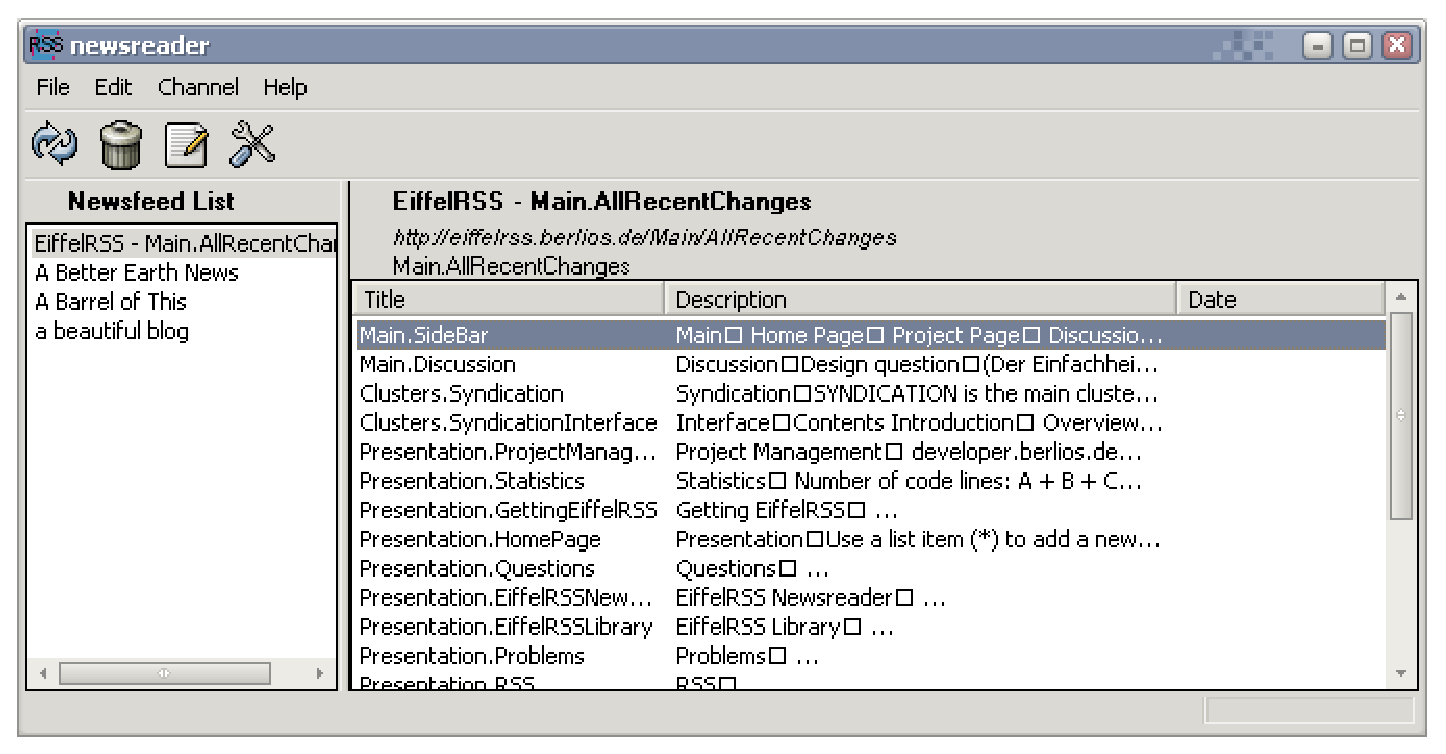
\includegraphics[width=0.95\textwidth]{./figures/main-window}
  \caption{Screenshot of the main window of Newsreader}
  \label{fig:main-window}
\end{figure}


\subsection{The Menu Bar}
\label{sec:menu-bar}

The menu bar consits of four items:

\begin{itemize}
\item File
\item Edit
\item Channel
\item Help 
\end{itemize}


\subsubsection{``File'' Menu}

In the ``File'' menu, there's just the option \textit{Exit}, which
will terminate the application.


\subsubsection{``Edit'' Menu}

In the ``Edit'' menu, you can access the preferences dialog with the
corresponding menu item.

\subsubsection{``Channel'' Menu}

This menu has several items.

\begin{itemize}
\item \textit{Add}: Show a dialog where you can enter an address to an
  RSS feed to add it to the subscribed feeds
\item \textit{Refresh}: Refresh the feed you are currently viewing
  (this will restore any deleted items, as long as they are still in
  the feed).
\item \textit{Feed information}: Show a dialog window with information
  about current feed
\item \textit{Item information}: Show a dialog window with information
  about the currently selected feed item
\item \textit{Remove feed}: Permanently remove the feed that is
  currently displayed
\item \textit{Remove item}: Remove the currently selected feed item
  (when the feed is refreshed, all items of the feed will be added
  again)
\item \textit{Refresh all}: Refresh all feeds
\end{itemize}

\subsubsection{``Help'' Menu}

The only item in this menu is \textit{About}, which will show you
information about the application's version and its developers.


\subsection{The Toolbar}
\label{sec:toolbar}

\begin{itemize}
\item[] 
\includegraphics[scale=0.4]{./figures/toolbar-refresh} $\;$
  Refresh all feeds
\item[] 
\includegraphics[scale=0.4]{./figures/toolbar-remove} $\;$
  Remove currently selected feed or item
\item[]
\includegraphics[scale=0.4]{./figures/toolbar-info} $\;$ Show
  dialog with information on currently selected feed or item
\item[] 
\includegraphics[scale=0.4]{./figures/toolbar-preferences}
  $\;$ Show preferences dialog
\end{itemize}


\subsection{The Feed List}
\label{sec:feed-list}

The feed list shows all subscribed feeds. When you click on one of
them, the feed detail view will show it's items.

Figure \ref{fig:feed-list} shows a screenshot of the feed list.

\begin{figure}[htbp]
  \centering
  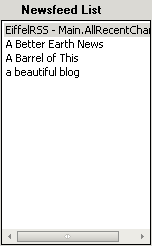
\includegraphics[scale=0.7]{./figures/feed-list}
  \caption{Screenshot of the feed list of Newsreader}
  \label{fig:feed-list}
\end{figure}


\subsection{The Feed Detail View}
\label{sec:feed-detail}

The feed detail view shows the items of the currently selected feed.
You can double click an item to open it in your browser. The title of
the current feed is shown at the top along with its link and
description.

Figure \ref{fig:feed-detail} shows a screenshot of the feed detail view.

\begin{figure}[htbp]
  \centering
  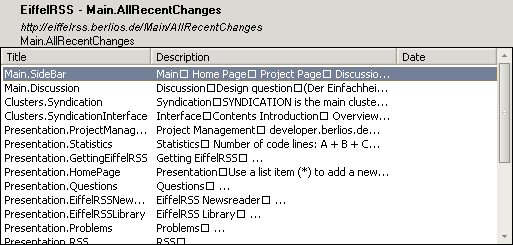
\includegraphics[scale=0.7]{./figures/feed-detail-view}
  \caption{Screenshot of the feed detail view of Newsreader}
  \label{fig:feed-detail}
\end{figure}


\section{Preferences Dialog}
\label{sec:preferences}

This is the place where you can configure Newsreader.

Figure \ref{fig:preferences} shows a screenshot of the preferences
dialog.

\begin{figure}[htbp]
  \centering
  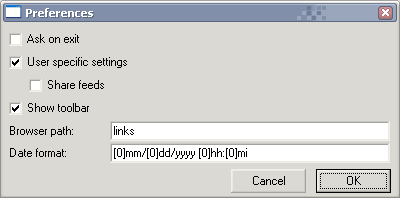
\includegraphics[scale=0.7]{./figures/preferences-dialog}
  \caption{Screenshot of the preferences dialog of Newsreader}
  \label{fig:preferences}
\end{figure}

The following options are available:

\begin{itemize}
\item \textit{Ask on exit}: When this check button is selected, a
  dialog will ask you whether you want to exit the application before
  it closes.
\item \textit{User specific settings}: When this check button is
  selected, Newsreader will save the preferences in a user specific
  file (Windows: \texttt{$\backslash$newsreader$\backslash$}, Unix:
  \texttt{/.newsreader/})
\item \textit{Share feeds}: When this check button is selected,
  Newsreader will not store the information about the subscribed feeds
  in a user specific file (This option is only available if
  \textit{User specific settings} is selected).
\item \textit{Show toolbar}: When this check button is deselected, the
  toolbar will be hidden.
\item \textit{Browser path}: Path to your browser executable.
\item \textit{Date format}: The format, in which the dates are shown.
\end{itemize}


\section{The Debug Window}
\label{sec:debug-window}

In the debug window, you can see the log of Newsreader (which is saved
to \texttt{newsreader.log}) and the preferences (select \textit{Show
  properties} to see them, and click \textit{Refresh} to update them).
You can disable the debug window with the command line argument
\texttt{-no\_debug\_window}.

Figure \ref{fig:debug-window} shows a screenshot of the debug window.

\begin{figure}[htbp]
  \centering
  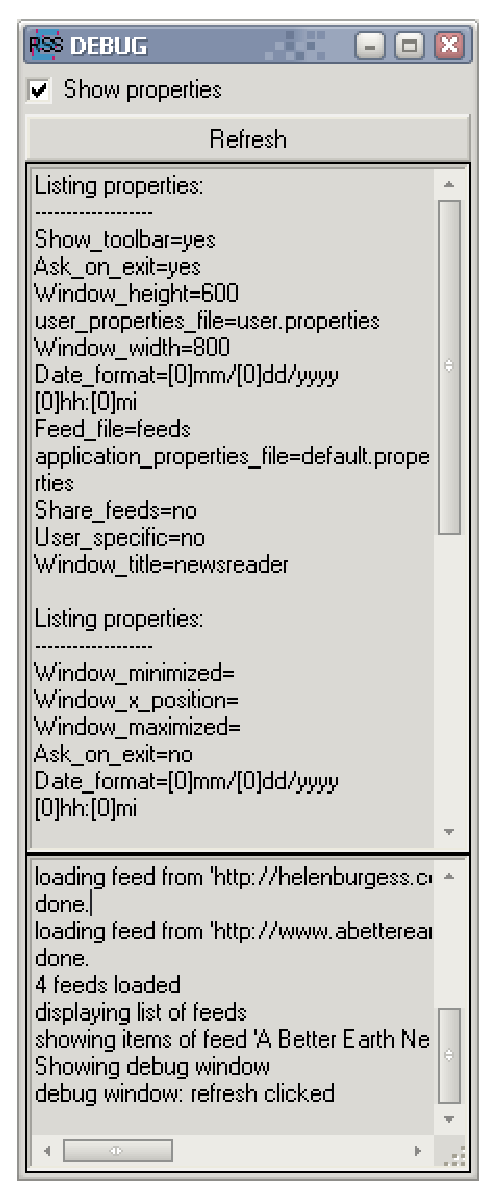
\includegraphics[scale=0.7]{./figures/debug-window}
  \caption{Screenshot of the debug window of Newsreader}
  \label{fig:debug-window}
\end{figure}

\section{The Command Line Version}
\label{sec:command-line}

There is a command line version of Newsreader, which can be started by
providing the command line parameter \texttt{-cl}. 

It is not feature complete, though. It is not possible to change
preferences and to add feeds (though you can add your feeds to the
\texttt{feeds} file). It just loads any feeds in the \texttt{feeds}
file. It is possible to see a list of feeds, a list of the items of a
feed, information on a feed or item and to open an item in your
browser (you could choose eg. \texttt{links} to open it directly in
the console).

Information on the available commands and their description are always
available with the \texttt{help} command.

\end{document}
